% !TEX root = ./0.main.tex

电子商务的发展近年来改变了我们的购物方式。推荐系统在电子商务公司中起着基础的作用。
传统的推荐方法主要使用协作过滤方法~\cite{sarwar2001item,schafer2007collaborative} 来预测用户和项目之间的得分。 最近,由于深度学习的快速发展,神经网络已广泛用于电子商务推荐系统。 神经推荐系统生成用户和项目的表示形式,且优于传统的推荐方法。但是,由于电子商务用户和商品的规模较大,因此很难使用深度模型直接给出每对用户和商品之间的点击率(CTR)预测。 目前的工业实践是使用快速k邻近算法 (例如, Faiss~\cite{JDH17}) 来生成候选项目,然后使用深度模型(例如, xDeepFM~\cite{lian2018xdeepfm}) 来集成用户和商品以优化业务指标(例如CTR)。

% \xz{The traditional way of building up such systems mainly relies on collaborative filters, while neural-network-based models are becoming more and more popular. Modern architecture first embeds users and items, then use fast matching algorithms like fast K nearest neighbors (Faiss~\cite{JDH17}) to match these embeddings, or use more complex ways that integrate the attributes of users and items to optimize the business metrics, like xDeepFM~\cite{lian2018xdeepfm}.  } 
% Recommender systems become a fundamental part of e-commerce companies. All sorts of recommendation algorithms play an essential role in recommender systems. Traditional recommendation methods mainly use collaborative filtering to predict scores between users and items and recommend users with high-score items. Recently, neural networks have been widely used in e-commerce recommender systems, which owe to the rapid development of deep learning. Neural recommendation methods generate representations for users and items and outperform traditional recommendation algorithms.

% As we can see, the function of neural networks is to obtain the item candidates instead of giving the final recommendation list for each user.
% \xz{The problem of neural-network-based models is that they require to run. If the number of users and items scale up tremendously, for example, billions of users and items, then there's still a large gap between embeddings and final recommendations.  } 
% Excessive item pool with billions of items limits the effects of neural networks. 
最近的一些工作利用图嵌入方法来获取用户和项目的表示,这些表示可用于下游应用程序。例如,PinSage~\cite{ying2018graph} 建立在 GraphSAGE~\cite{hamilton2017inductive} 的基础上,并将基于图卷积网络的方法应用于具有数十亿个节点和边的生产规模数据。GATNE~\cite{cen2019representation} 考虑了不同的用户行为类型,并利用异构图嵌入方法来学习用户和项目的表示。 但是,这种方法忽略了用户行为中的顺序信息,并且无法捕获相邻用户行为之间的相关性。 %Also, user behaviors are updated in real time, so recommendation methods should give real-time recommendations for all users. 

最近的研究~\cite{kang2018self,chen2018sequential,lv2019sdm} 将推荐系统形式化为顺序推荐问题。根据用户的行为历史记录,顺序推荐任务是预测他/她可能感兴趣的下一个项目。此任务反映了现实中的推荐系统的情况。许多最新模型可以根据其行为顺序为每个用户提供整体嵌入。但是,统一的用户嵌入很难代表多个兴趣。 例如,在图~\ref{fig:multiple_interest} 中,单击序列显示了Emma的三种不同兴趣。 作为一个现代女孩,Emma 对珠宝,手袋和化妆品感兴趣。 因此,在这段时间,她可能单击三个类别的项目。

% \begin{figure}
%     \centering
%     \includegraphics[width=0.45\textwidth]{figures/multiple_interests.pdf}
%     \caption{An example click sequence of a e-commerce user, Emma. The click sequence indicates that Emma has multiple interests including clothes, handbags, and makeups.}
%     \label{fig:multiple_interest}
% \end{figure}

\begin{figure*}
    \centering
    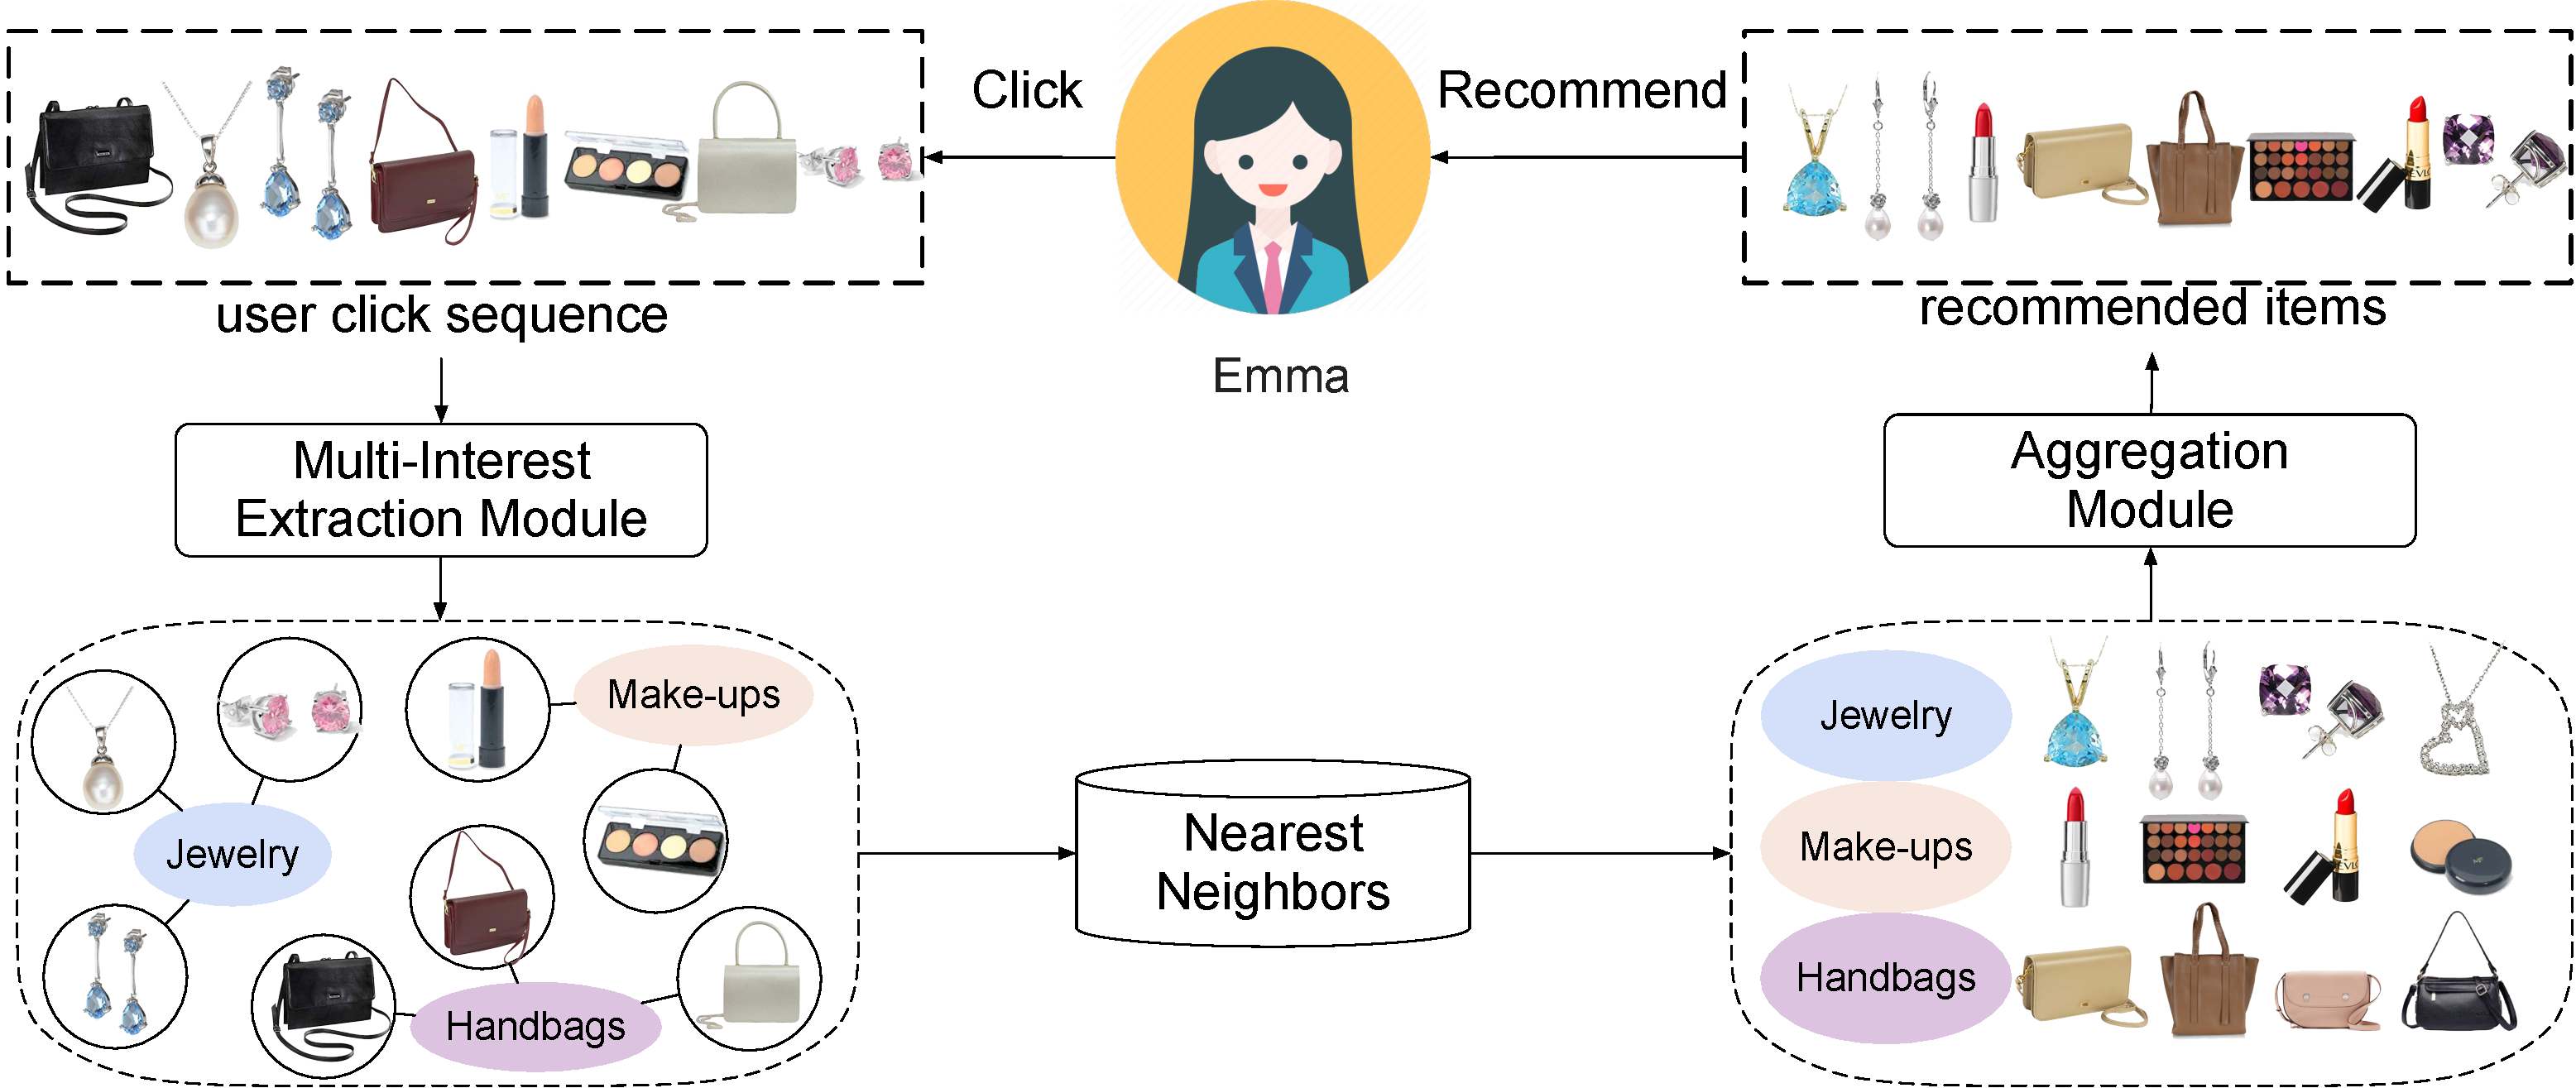
\includegraphics[width=0.8\textwidth]{figures/multi-interest-overview.pdf}
    \caption{我们提出的框架的一个令人振奋的例子。 电子商务平台用户Emma具有多种兴趣,包括珠宝,手袋和化妆品。 我们的多兴趣提取模块可以从她的点击序列中捕获这三个兴趣。 每个兴趣都基于兴趣嵌入独立地从大型项目池中检索项目。 汇总模块组合了来自不同兴趣的项目,并输出Emma推荐的总体前N个项目。 }
    \label{fig:multiple_interest}
\end{figure*}

在本文中,我们提出了一种新的可控多兴趣框架 \model。我们的多兴趣模块可以捕获用户的多个兴趣,可以将其用于检索候选项目。我们的汇总模块将这些来自不同兴趣的项目组合在一起,并输出总体建议。图~\ref{fig:multiple_interest} 显示了我们的多兴趣框架的一个令人振奋的例子。我们针对顺序推荐进行实验,这与我们的在线情况类似。实验结果表明,我们的框架优于其他最新模型。我们的框架也已成功部署在阿里巴巴分布式云平台上。十亿规模的工业数据集上的结果,进一步证实了我们的模型在实践中的有效性和效率。

总而言之,本文的主要贡献有:
\begin{itemize}
    \item 我们提出了一个综合框架,该框架将可控性和多兴趣组件集成在一个统一的推荐系统中。
    \item 我们通过实施和研究在线推荐方案来研究可控性在个性化系统上的作用。
    \item 我们的框架在两个具有挑战性的真实数据集上实现了最先进的性能,可进行顺序推荐。
\end{itemize}

\iffalse
\begin{itemize}
    \item We propose a novel controllable multi-interest framework based on user sequential behaviors for sequential recommendation.
    \item The controllable module in our framework can adjust the diversity of recommended item candidates. 
    % \item We adapt the capsule network with a variation of the dynamic routing method for the multi-interest extraction. 
    \item Our framework achieves state-of-the-art results on two real-world datasets for sequential recommendation.
    % \item CapsRec has been deployed on Alibaba recommender systems and significantly improves hit rate on a billion-scale industrial dataset. 
\end{itemize} 
\fi


% \vpara{Organization}
% The rest of the paper is organized as follows. Section~\ref{sec:related} summarizes related work. Section~\ref{sec:model} formulates the sequential recommendation problem and introduces our proposed framework in detail. In Section~\ref{sec:exp}, we conduct extensive experiments and case studies. Finally, we conclude in Section~\ref{sec:conclusion}.
%% vim: formatoptions=
